\section{Dimensionality Reduction}
Ragionamento: I dati N-dimensionali vengono proiettati in 2 o 3 dimensioni per una migliore visualizzazione/comprendimento.
Strategia ampiamente utilizzata.
In generale, si tratta di un mapping e non di una trasformazione geometrica.
Diversi mappings presentano diverse proprietà.
\subsection{Principal Component Analysis (PCA)}
Una tecnica classica per la riduzione della dimensione è la \textbf{Principal Component Analysis (PCA)}.
Si tratta di una tecnica lineare e non parametrica, l'idea principale è trovare una base formata da delle direzioni che massimizzano la varianza dei dati.
L'idea è di rappresentare i dati in nuova base che meglio \textit{esprime} i nostri dati.
La nuova base è una combinazione lineare della base originale.
\begin{figure}[H]
    \centering
    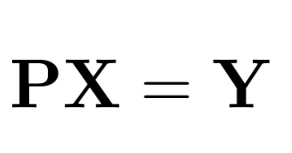
\includegraphics[width=0.5\textwidth]{images/Basis.png} 
    \caption{Cambio di Base}
    \label{fig:immagine}
\end{figure}
\subsubsection{Signal-to-noise Ratio (SNR)}
\begin{figure}[H]
    \centering
    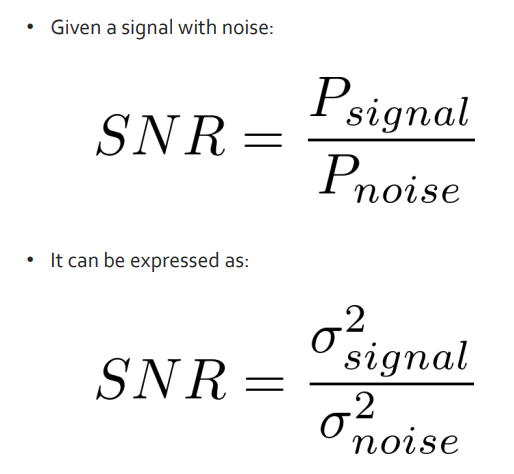
\includegraphics[width=0.5\textwidth]{images/Radio.png} 
    \caption{Basis}
    \label{fig:immagine}
\end{figure}
\subsection{Covariance Matrix \& Risolvere PCA}
Cov(x)=....
Matrice quadrata simmetrica, gli elementi sulla diagonale corrispondono alla varianza di una particolare variabile.
Come selezionare la \textbf{P} migliore per il cambio di base?
Quella che minimizza la ridondanza e che massimizza la varianza.
L'obbiettivo è diagonalizzare la matrice della covarianza di Y.
Valori alti sulla diagonale significano che la "dinamica" della singola variabile è stata massimizzata.
valori bassi dei valori che non si trovano sulla diagonale significa che la ridondanza tra le variabili è minimizzata.
\textbf{Theorem}: una matrice simmetrica A può essere diagonalizzata da una matrice formata dai suoi autovettori
come A=EDE', dove le colonne di E sono gli autovettori di A.
Quindi si organizzano i dati come una matrice mxn, si sottrae la media corrispondente ad ogni riga
si calcolano gli autovettori e gli autovalori della matrice XX'
e infine si organizzano per formare la matrice P
L'idea è trovare la k-esima componente principale, proiettare i dati in queste direzioni e usare questi dati invece di quelli originali.
Questi dati sono la migliore approssimazione rispetto alla somma dei quadrati delle differenze.
\subsubsection{limit of PCA}
Uno dei limiti è che la funzione non è parametrica -> è sia un punto forte che un punto debole
Non funziona per i dati che non seguono una distribuzione gaussiana, può essere estesa per prendere in considerazione anche le trasformazioni non lineri.
\subsubsection{PCA and MDS}
\subsection{Locally Linear Embedding}(LLE)
\textbf{LLe} cerca di scoprire strutture non lineari in grandi dimensioni sfruttando le approssimazioni lineari locali.
\begin{figure}[H]
    \centering
    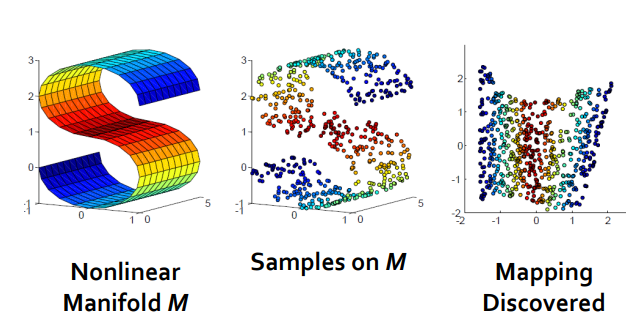
\includegraphics[width=0.5\textwidth]{images/LLe.png} 
    \caption{Locally Linear Embedding}
    \label{fig:immagine}
\end{figure}
Assumendo che ci sono dati suffcienti, ci aspettiamo che ogni punto e i suoi vicini possono essere approssimati da una patch lineare locale.
La patch è rappresentata dalla somma pesata dei punti locali.
Prendi un insieme di dati vicino ad un punto(ball-radius)
e risolvi per Wij.
.....
Trova il vettore Yi che minimizza la funzione di costo (embedding).
\begin{itemize}
    \item 1. Calcola i vicini di ogni data point Xi.
    \item 2. Calcola i pesi che meglio ricostruiscono Xi.
    \item 3. Calcola i vettori che minimizzano la funzione di costo.
\end{itemize}
\subsection{ISOMAP}
L'idea principale è quella di preservare la distanza geodesica tra due punti
La distanza geodesica la distanza più breve tra due punti in uno spazio curvo.
\begin{figure}[H]
    \centering
    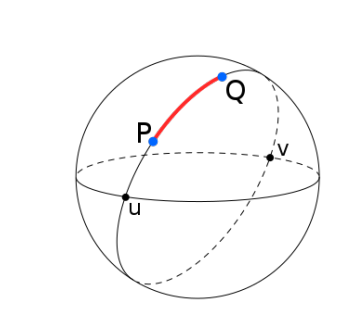
\includegraphics[width=0.5\textwidth]{images/geod.png} 
    \caption{Geodesic distance}
    \label{fig:immagine}
\end{figure}
\begin{itemize}
    \item 1. Costruire il grafo dei vicini.
    \item 2. Calcola il path più breve.
    \item 3. Costruisci il d dimensional embedding(?).
\end{itemize}
\begin{figure}[H]
    \centering
    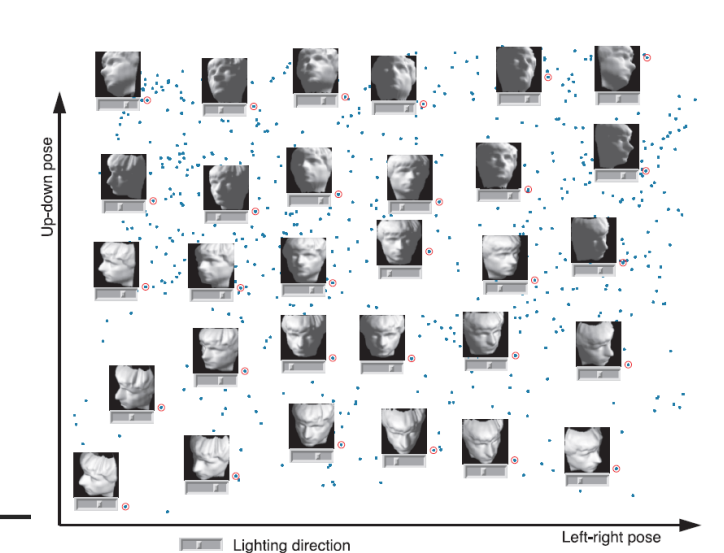
\includegraphics[width=0.5\textwidth]{images/ISOMAP.png} 
    \caption{Geodesic distance}
    \label{fig:immagine}
\end{figure}
\subsection{Autoencoders}
Il Machine Learning ormai è presente in ogni ambito dell'inforamtica, un tipo speciale di neural network è chiamatao \textbf{Autoencoder}.
Un autoencoder può essere usato per la dimensionality reduction
\begin{figure}[H]
    \centering
    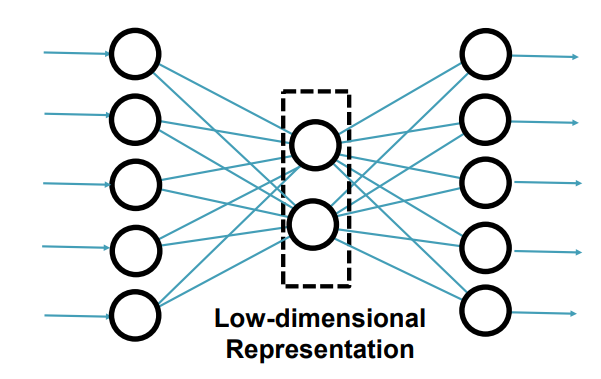
\includegraphics[width=0.5\textwidth]{images/Autoencoders.png} 
    \caption{Geodesic distance}
    \label{fig:immagine}
\end{figure}
\subsection{SNE, Stocastic Neighbor Embedding}
Molte tecniche per la riduzione della dimensione non sono utili per restituire sia la struttura locale che quella globale dei dati in una singola mappa.
Le Similarità tra  high and low dimensional data points sono modellate con le condizioni di probabilità
...
